\chapter{Grundlagen}
\label{chapter:grundlagen}

Im folgenden Kapitel werden die Begriffe Event, Stream, Processing aus der Informatik im Bereich der verteilten Systeme erläutert und in einen Zusammenhang zu Streaming frameworks gebracht. Dabei wird ein Grundkonzept für eine streambasierte Nachrichtenverarbeitung vorgestellt. Im weiteren Verlauf und maßgeblich in Kapitel \ref{chapter:vorstellung} wird stets auf das Grundkonzept Bezug genommen. In der Einführung wurde die stream processing engine Borealis \citelit{abadi2005design} als ein einfaches Modell eines Stream processing-Systems erwähnt. Zuerst werden im Unterkapitel \ref{section:grundbegriffe} die wesentlichen Fachbegriffe vorgestellt. Anschließend wird im Unterkapitel \ref{section:technologie} ein Zeitbezug zu verwandten Technologien gegeben und die Streaming frameworks aus Kapitel \ref{chapter:vorstellung} werden eingeordnet. Das Kapitel \ref{chapter:grundlagen} endet mit einer Zusammenfassung und leitet in das Kapitel \ref{chapter:analyse} ein.

\section{Grundbegriffe}
\label{section:grundbegriffe}

Ein großer Teil der verwendeten Grundbegriffe sind in \citelit{tanenbaum:vs} definiert. An dieser Stelle werden nur die wesentlichen Grundbegriffe vorgestellt.
Ein Verteiltes System wird von Andrew S. Tanenbaum und Maarten van Steen in \citelit[S. 19, K 1.1]{tanenbaum:vs} grob definiert:

\begin{quote}
Ein verteiltes System ist eine Ansammlung unabhängiger Computer, die den Benutzern wie ein einzelnes kohärentes System erscheinen.
\end{quote}

Verteilte Systeme bestehen also laut \citelit{tanenbaum:vs} aus unabhängigen Komponenten und enthalten eine bestimmte Form der Kommunikation zwischen den Komponenten. Informationen werden zwischen Sender und Empfänger über ein Signal ausgetauscht. Dazu hat Claude E. Shannon in \citelit[S. 2, A. 1]{shannon1948} ein Diagramm eines allgemeinen Kommunikationssystems vorgestellt. In der genannten Abbildung wird das Signal in einem Kanal codiert übertragen. Dabei ist das Signal einem Umgebungsrauschen ausgesetzt. Durch Einsatz geeigneter Kodierverfahren in Übertragungsprotokollen können Übertragungsfehler festgestellt und behoben werden. Im schlimmsten Fall wird eine fehlerhaft übertragene Nachricht zum Beispiel innerhalb des \gls{glo:tcp} auf OSI Schichtebene 4 in \citelit[S. 40, K. 7.4.4.6 Data transfer phase]{itux200} neu übertragen. Der Kanal ist das Medium in \citelit{shannon1948}, um die Nachricht zu übertragen. %% Signalarten
Tanenbaum und van Steen beschreiben in \citelit[S. 184, K. 4.4.1]{tanenbaum:vs} ein kontinuierliches Medium Temperatursensor gegenüber einem diskreten Medium Quelltext als zeitkritisch zwischen Signalen. %Außerdem ist die Reihenfolge bei Audiosignalen für eine richtige Interpretation wichtig.
Shannon beschreibt in \citelit[S. 3 und S. 34]{shannon1948} ein kontinuierliches System als:

\begin{quote}
A continuous system is one in which the message and signal are both treated as continuous functions, e.g., radio or television. [...]
An ensemble of functions is the appropriate mathematical representation of the messages produced by
a continuous source (for example, speech), of the signals produced by a transmitter, and of the perturbing
noise. Communication theory is properly concerned, as has been emphasized by Wiener, not with operations
on particular functions, but with operations on ensembles of functions. A communication system is designed
not for a particular speech function and still less for a sine wave, but for the ensemble of speech functions.
\end{quote}

Ein Stream oder ein Datastream ist damit eine Folge von Signalen. Einem Signal entspricht ein Event und die Anwendung von Funktionen findet im Processing statt. Somit ist Event stream processing eine Signalfolgenverarbeitung in einem kontinuierlichen Medium. Weiterhin soll in diesem Zusammenhang von Event stream processing oder abgekürzt \acrshort{glo:esp} benutzt werden.

Da zu Streams ebenfalls eine Paketierung von unterschiedlichen Substreams aus Audio, Video und Synchronisierungsspezifikation verstanden wird, wie in \citelit[S. 191, letzter Absatz]{tanenbaum:vs} mit dem Kompressionsverfahren 2 und 4 für Audio und Video Übertragung der \gls{glo:mpeg} gezeigt, soll an dieser Stelle keine tiefergehende Untersuchung in den Zusammenschluss unterschiedlicher Algorithmen zur Komprimierung der Substreams in einen Stream erfolgen. 

Weiterhin beschreibt Muthukrishnan in \citelit{research:massivedata} (2010) mehrere Forschungsrichtungen in Datastreams. Darunter werden "`[...] theory of streaming computation [...], data stream management systems [...], theory of compressed sensing [...],"' \citelit[S. 2, Absatz 2]{research:massivedata}  aufgezählt. In \textit{streaming computation} wird an geringen Zugriffszeiten während mehrfachem Zugriff auf gegebener Datennachrichten geforscht. 
Mit einem \textit{data stream management system} soll ein Zugriff, durch Einsatz von speziellen Operatoren auf nicht endende Datenquellen möglich sein. Und in der \textit{theory of compressed sensing} wird nach geringen Zugriffsraten zum Aufteilen in Signalmustern unterhalb der Nyquist-Rate geforscht. So findet Streaming in der Signalverwaltung, Signalverarbeitung und Signaltheorie eine Anwendung.

% (1) basic terminology, (2) measures of event processing performance,
% (3) streams dienstgüte (Pünktlichkeit, Umfang, Zuverlässigkeit): qos

Während Streams auf einem Prozessorsystem verarbeitet werden können, muss eine hohe Kapazität von Daten auf einem oder mehreren Multiprozessorsystemen in einer geringen Latenz verteilt berechnet werden können. Tanenbaum und van Steen stellen die Grundlagen der \gls{glo:rpc}-Verwendung in \citelit[S. 150, K. 4.2.1]{tanenbaum:vs} vor. Abstraktionen der Schnittstelle zur Transportebene, wie diese auf OSI Ebene 4 durch \gls{glo:tcp} angeboten werden, bilden dabei eine Vereinfachung um Funktionen mit übergebenen Parametern auf entfernten Rechnern aufzurufen. Nach der entfernten Berechnung wird das Ergebnis sofort an den Client zurückgeschickt. Dabei ist der Client bei einem synchronen Nachrichtenmodell blockiert bis der Server geantwortet hat. Sobald die Berechnung durchgeführt wurde, wartet im asynchronen Nachrichtenmodell der Client nicht und wird erst nach Abschluß der Berechnung am Server vom Server informiert. Währenddessen können weitere Anfragen durch den Client auf den Server erfolgen. 

Wie in \citelit[S. 170, K. 4.3.2]{tanenbaum:vs} vorgestellt, wurde durch den Einsatz von Warteschlangensystemen ein zeitlich lose gekoppelter Nachrichtenaustausch zwischen Sender und Empfänger möglich. Der Empfänger entscheidet selbst wann und ob eine Nachricht eines Senders von der Warteschlange abgeholt wird. Zusätzlich entsteht die Möglichkeit des Warteschlangensystems Nachrichten zwischenzuspeichern. Im Gegensatz zu \glspl{glo:rpc} haben Nachrichten in Warteschlangensystemen eine Adresse und können beliebige Daten enthalten. 
% Grafik Client/Server

Mehrere Server in einem Verbund bilden ein Cluster. In einem Cluster übernehmen einzelne Rechner-Knoten die Berechnung. Außerhalb der Rechner-Knoten gibt es einen Master-Knoten mit dem die Rechenaufgaben auf die Rechner-Knoten verteilt werden. Dazu wird von Tanenbaum und van Steen in \citelit[S. 35, A. 1.6]{tanenbaum:vs} ein Cluster-Computersystem in einem Netzwerk gezeigt. Diese Prinzip wird auch in den Streaming frameworks eingesetzt. In dem Kapitel \ref{chapter:vorstellung} werden die einzelnen Frameworks im Detail vorgestellt. Die Streaming frameworks selbst bieten dabei ähnlich wie es bei den \glspl{glo:rpc} der Fall ist, eine Abstraktionsschicht um die Datenverarbeitung für den Entwickler zu vereinfachen. Dazu werden abstrakte Primitive und Operatoren für die Anwendung auf einem unterliegenden Cluster bereitgestellt.

Es wurden die Grundbegriffe eines Streaming Frameworks vorgestellt und eingeordnet. In Kapitel \ref{section:technologie} wird ein Basis Streaming Framework als Modell vorgestellt. Außerdem werden die Streaming Frameworks Storm, Kafka, Flume und S4 kurz zum Basis Streaming Framework Modell in Zusammenhang gebracht. Die Technologie die dazu zum Einsatz notwendig ist, wird in eigenen Unterkapiteln vorgestellt.

\section{Technologie}
\label{section:technologie}

Mit den gewonnen Grundbegriffen werden in diesem Kapitel ein Modell eines Basis Streaming framework vorgestellt. Zuerst wird das Grundmodell und deren Komponenten gezeigt und beschrieben. Anschließend werden die Straming frameworks Storm, Kafka, Flume und S4 mit dem Modell des Streaming frameworks in eine Beziehung gebracht und erläutert. Das Unterkapitel \ref{section:technologie} endet mit weiteren Komponenten für Streaming frameworks und leitet in das Unterkapitel \nameref{section:zusammenfassung} ein.

%\subsection{Basis Modell für Streaming frameworks}
%\label{subsection:basismodel}

Ein Basis Modell für Streaming frameworks soll durch eine \gls{glo:spe} Aurora/Borealis \citelit{auroraNewModelAndArchitecture} veranschaulicht werden. Im weiteren Verlauf wird zur Vereinfachung das Schlagwort \textit{Aurora} anstatt \gls{glo:spe} Aurora/Borealis verwendet. So besteht ein Modell in \citelit[S. 2, Abb. 1 Aurora system model]{auroraNewModelAndArchitecture} aus ankommenden Daten, den \textit{Input data streams}, aus ausgehenden Daten, dem \textit{Output to applications} und aus wiederkehrenden Abfragen, den \textit{Continous queries}. In Abbildung \ref{fig:basismodell} wird ein Modell als Grundlage für weitere Betrachtungen zu Streaming frameworks vorgestellt. Dabei wird ein azyklisch gerichteter Graph im Zentrum als Verarbeitungseinheit mit linker und rechter Datenflussüberführung gezeigt.

\begin{figure}[htb!]
\centering
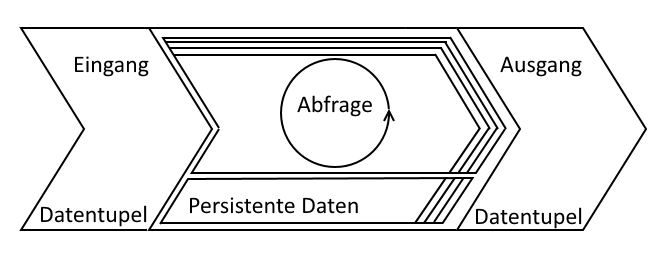
\includegraphics[width=1.0\textwidth]{bilder/StreamingFrameworkBasisModell.png}
\caption{Exemplarische Darstellung eines Basis Modells für Streaming frameworks
\label{fig:basismodell}}
\end{figure}

Dabei sind \textit{Input data streams} eine Sammlung von Werten und werden von \textit{Aurora} als eindeutiges Tupel mit einem Zeitstempel identifiziert. Innerhalb von \textit{Aurora} können mehrere \textit{Continous queries} gleichzeitig ausgeführt werden. Abbildung \ref{fig:basismodell} stellt in der Mitte der Grafik zwischen Eingang und Ausgang der Datentupel mehrschichtige Ebenen als Repräsentation für mehrere \textit{Continous queries} dar.

Ein \textit{Continous query} besteht aus \textit{boxes }und \textit{arrows}. \textit{Boxes} sind Operatoren um ankommende Datentupel in ausgehende Datentupel zu überführen. Durch die \textit{Arrows} wird eine Beziehung zwischen den \textit{Boxes} hergestellt. Ein komplexer Beziehungsgraph ist in eine Richtung gerichtet, enthält keine Zyklen, hat mehrere Startknoten und einen Endknoten. Für die weitere Datenverarbeitung können in einem \textit{Continous query} zusätzlich persistente Datenquellen in einer \textit{Box} zur Transformation von Datentupeln hinzugefügt werden. Dazu wird in Abbildung \ref{fig:basismodell} unterhalb der \textit{Continous queries} ein mehrschichtiger separater Bereich für die persistenten Daten dargestellt. Im Endknoten des azyklisch gerichteten Graphen werden die transformierten Datentupel für weitere Anwendungen als Ausgabestrom von Datentupeln bereitgestellt. Die Abbildung \ref{fig:dag} stellt beispielhaft einen azyklisch gerichteten Graphen dar. Der dargestellte Graph enthält zwei Eingangdatenquellen. Die obere Datenquelle wird zeitlich kurz vor dem Endknoten mit der unteren Datenquelle kombiniert. Die unter Datenquelle enhält wird nach der zweiten Transformation in zwei neue Datenquellen aufgespalten. Nach drei Transformationen wird die mittlere Datenquelle in die oberer Datenquelle zeitlich an der sechsten Transformation überführt. Die untere Datenquelle wird mit der oberen Datenquelle an der siebten Transformation verbunden. Die letzte Transformation bildet den Endknoten.

\begin{figure}[htb!]
\centering
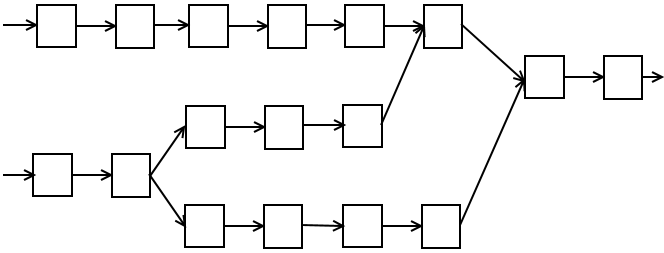
\includegraphics[width=1.0\textwidth]{bilder/DAG.png}
\caption{Darstellung eines azyklisch gerichteten Graphen
\label{fig:dag}}
\end{figure}

Das Datenmodell in \textit{Aurora} besteht aus einem \textit{Header}, dem Kopfbereich und Data, dem Datenteil als Tupel. Der Header in einem Basismodell besteht aus einem Zeitstempel. Mit dem Zeitstempel wird das Datenpaket eindeutig identifiziert und wird für das Monitoring in \gls{glo:qos} als einen Dienst für die Güte eingesetzt. Im Gegensatz zu \textit{Aurora} wird in der auf \textit{Aurora} basierten Weiterentwicklung \textit{Borealis} ein Vorhersagemodell für \gls{glo:qos} zu jedem Zeitpunkt in einem Datenfluss möglich. Dazu wird jedem Datentupel ein \gls{glo:vecme} hinzugefügt. Ein \gls{glo:vecme} besteht aus weiteren Eigenschaften wie zum Beispiel Ankunftszeit oder Signifikanz. In \citelit[S. 3, Kap. 2.4 QoS Model]{abadi2005design} werden \acrlong{glo:vecme} vorgestellt.


In \textit{Borealis} gibt es statuslose Operatoren und Operatoren mit einem Status. Statuslose Operatoren sind Filter, Map und Union. Mit dem Filter kann eine Datenquelle nach bestimmten Bedingungen neue Datenquellen erzeugen. Der Map-Operator kann bestimmte Datentupel in einer Datenquelle transformieren wie zum Beispiel durch anreichern von Informationen. Mit dem Union-Operator können mehrere Datenquellen in eine Datenquelle zusammengeführt werden. Dazu wird ein Zwischenspeicher in der Größe n + 1 benutzt. In \citelit[S. 9, Abb. 3.1 Sample outputs from stateless operators]{borealis:programmer} wird eine Übersicht über die drei Operatoren Filter, Map und Union anhand eines konkreten Beispiels dargestellt. Operatoren mit einem Status wie \textit{Join} und \textit{Aggregate} werden in \cite[S. 9, Kap. 3.2.2 Stateful Operators]{borealis:programmer} als Berechnungen von speziellen Zeitfenstern, dem \textit{window}, die mit der Zeit mitbewegen erläutert. In \cite[S. 10, Abb. 3.2 Sample output from an aggregate operator]{borealis:programmer} wird ein Schaubild zum Operator \textit{Aggregate} mit der Funktion \textit{group by}, \textit{average} und \textit{order} in einem \textit{window} gezeigt. Dabei werden eingehende Datenquellen mit einem Schema nach Zeit, Ort und Temperatur in einem Zeitfenster von einer Stunde gruppiert nach Raum, gemittelt nach Temperatur und sortiert nach Zeit in eine ausgehende Datenquelle transformiert. In Abbildung \ref{fig:querydiagramspe} wird ein Abfrage-Diagramm in einer \acrlong{glo:spe} dargestellt. Es werden zwei Sensoren S1 und S2 mit dem Union-Operator in einen Stream zusammengeführt. Der Stream wird von zwei Aggregate-Operatoren in einem Zeitfenster von 60 Sekunden getrennt und jeweils mit einem Filter-Operator reduziert. Durch den Join-Operator werden beide Stream in einem Zeitfenster von 60 Sekunden zu einem dritten Stream transformiert.

\begin{figure}[htb!]
\centering
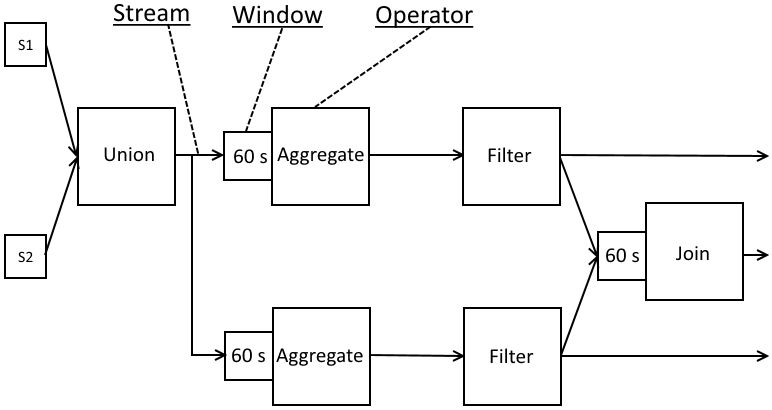
\includegraphics[width=1.0\textwidth]{bilder/QueryDiagram.png}
\caption{Diagramm einer Abfrage in einer \acrlong{glo:spe}
\label{fig:querydiagramspe}}
\end{figure}

Datentupel in \textit{Aurora} können aufgrund von technischen Fehlern, wie zum Beispiel Sensorausfall oder doppelter Parametrierung von mehreren Sensoren durch Hinzufügen, Löschen oder Aktualisieren verschiedene Versionen annehmen. Daher wurde das Datenmodell in \textit{Borealis} im \textit{Header} um einen Revisionstyp und einem Index erweitert. In separaten Speichern den \glspl{glo:cp} werden die Revisionen der Datentupel als Historie gehalten. Die \glspl{glo:cp} sind direkt an einer Datenquelle angeschlossen. Operatoren können auf die \glspl{glo:cp} durch die Identifikatoren im \textit{Header} auf benötigte Datentupel in der Historie zugreifen.

In den Streaming frameworks Storm, Kafka, Flume und S4 wird eine ähnliche Architektur wie sie im Referenzmodel von \textit{Aurora} und \textit{Borealis} vorgestellt wurde benutzt. Zwischen den Streaming frameworks gibt es trotzdem Unterschiede. Das Referenzmodell von \textit{Aurora} und \textit{Borealis} soll dem Verständnis bei der Vorstellung der Streaming frameworks im Kapitel \ref{chapter:vorstellung} dienen und die Unterschiede aufzeigen. Mit der Einführung der Grundbegriffe und eines Referenzmodells soll nun das Kapitel \nameref{chapter:grundlagen} im Unterkapitel \ref{section:zusammenfassung} zusammengefasst werden.

\section{Zusammenfassung}
\label{section:zusammenfassung}

Im Kapitel \nameref{chapter:grundlagen} wurden die Streaming frameworks in die Bereiche der Informationsverarbeitung in verteilten Systemen, der Signaltheorie und der wiederkehrenden Berechnung von Daten in Datenströmen eingeordnet. Dabei wurden aktuelle Forschungsbereiche aufgezeigt und es wurde ein Referenzmodell als Grundlage dargestellt. In der Beschreibung des Referenzmodells wurden die Primitive und die komplexen Operatoren vorgestellt. Weiterhin wurde ein Abfrage-Diagramm anhand eines azyklisch gerichteten Graphen gezeigt. Mögliche Fehlererkennung durch Qualitätssicherungsmaßnahmen wurden durch \acrlong{glo:vecme} angesprochen. Fehlererkennungsmechanismen und Gütesicherung werden im Einzelnen im Kapitel \ref{chapter:vorstellung} aufgezeigt. Bevor die Streaming frameworks vorgestellt werden, wird in Kapitel \ref{chapter:analyse} die Umgebung und der Markt analysiert.